\begin{figure}
\begin{center}
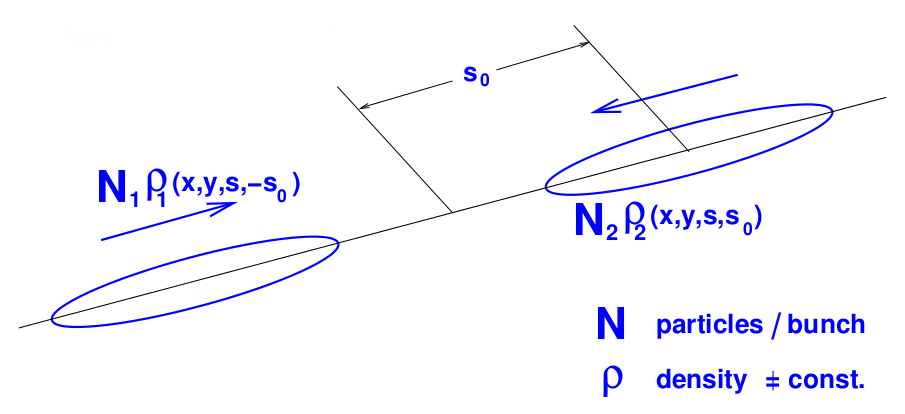
\includegraphics[width=\linewidth,height=\textheight,keepaspectratio]{../HourglassCorrection/figs/simple_bunch_head_on}
\caption{ 
Here we see two bunches colliding head on, which is a simplified model used to
estimate the expected luminsoity, before the application of the $\beta^{*}$
squeezing effect and any existence of crossing angles, $\theta_{XZ}$ or
$\theta_{YZ}$ 
}
\label{fig:simple_bunch_head_on}
\end{center}
\end{figure}
